%Para compilar pdflatex -shell-escape archivo.tex (en consola)
\documentclass[12pt]{article}
\usepackage{moodle}
\usepackage{graphicx}

\begin{document}
\begin{quiz}{Primer examen}

\begin{numerical}{Basic addition}
What is $8+3$?
\item 11
\end{numerical}
\begin{shortanswer}[case sensitive=true]{Newton’s name}
What was Newton’s first name?
\item Isaac
\item[fraction=0, feedback={No, silly!}] Fig
\item{fraction=0} Sir
\end{shortanswer}
\begin{multi}{A first derivative}
What is the first derivative of $x^3$?
\item $\frac{1}{4} x^4+C$
\item* $3x^2$
\item $51$
\end{multi}
%Si su pregunta es de opción multiple y es de varias opciones, recuerde colocar un valor negativo a todas las respuestas incorrectas, de lo contrario, el estudiante aprobará marcando todas.
\begin{multi}[multiple]{Pregunta2}
Which numbers are prime?
\item* 5
\item[fraction=-50] 6
\item* 7
\item[fraction=-50] 8
\end{multi}

%Otra categoria
\setcategory{Preguntas Q2}


\begin{essay}[response format=file,attachments allowed=1]{Hola}
Hola hábia una vez un bárco ñuno
\begin{center}
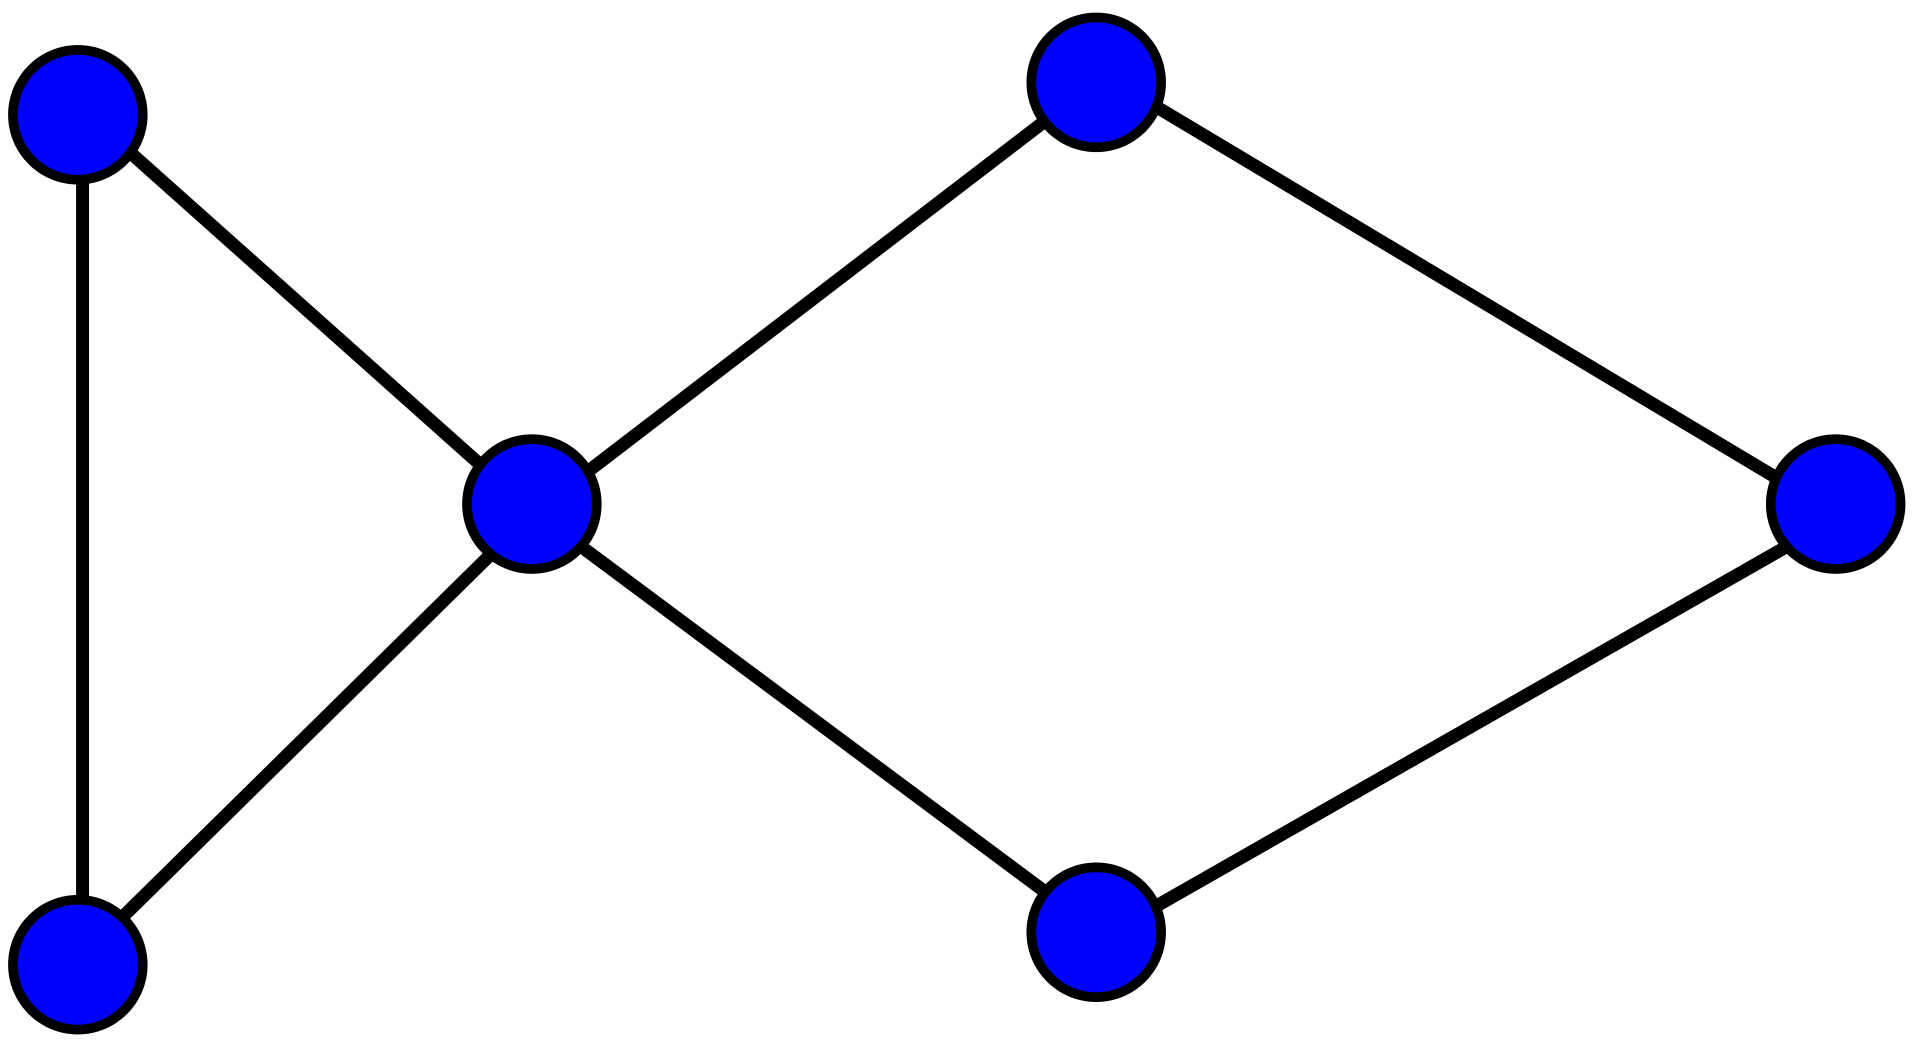
\includegraphics[width=4cm,height=4cm,ppi=100]{imagenes/grafo.png}
\end{center}
\item hnotes for grader i
\item hnotes for grader i
\end{essay}
\begin{multi}{my question}
Compute $\int 4x^3\,dx$.
\item* $x^4+C$
\item[fraction=50] $x^4$
\item $12x^2$
\end{multi}
\end{quiz}

\end{document}



